%%%----------SETUP----------%%%

\documentclass[11pt, titlepage]{article}
\usepackage{lmodern}
\usepackage[margin=1.25in, headheight=14pt]{geometry}
\usepackage{setspace}
    \onehalfspacing
\usepackage[dvipsnames]{xcolor}
\usepackage{tabularray}
\usepackage{nameref}
\usepackage{fancyhdr}
\usepackage[style=apa]{biblatex}
    \addbibresource{references.bib}
\usepackage[colorlinks=true, 
            allcolors=RoyalBlue,
            citecolor=.]{hyperref} 
\usepackage{graphicx}
    \graphicspath{ {images/} }


%%  Set biographic information for the title page and document

\newcommand{\thesistitle}{Thesis Title}
\newcommand{\thesisauthor}{Thesis Author}
\newcommand{\graddate}{Month and Year}
\newcommand{\facultyadvisor}{Faculty Advisor Name}
\newcommand{\preceptor}{Preceptor Name}
\newcommand{\keywords}{Key1; Key2; Key3...}

%% Set PDF metadata
\hypersetup{
  pdfauthor={\thesisauthor \ Copyright \textcopyright \number\year},
  pdftitle={\thesistitle},
  pdfsubject={MACSS MA Thesis},
  pdfkeywords={\keywords}
  pdfborder={0 0 0}
}

%% set up header footer style
\pagestyle{fancy}
\fancyhead{}
\fancyhead[R]{\thesisauthor}
\fancyfoot{}
\fancyfoot[C]{\thepage}




\begin{document}



\begin{titlepage}
    %% Do not edit the titlepage section. Make any changes above
    \begin{center}
        \vspace*{-0.45in}
        
\includegraphics[height = 1.5in]{images/Shield.png}\\
	\vspace{0.1in}
        \Large{\uppercase{The University of Chicago}}\\
	\vspace{0.8in}
	\LARGE{\textsc{\thesistitle\\}}
	\vspace{0.8in}
	\normalsize{By}\\
	\Large{\thesisauthor\\
	\vspace{0.5in}
	\graddate\\}
        \vspace{0.8in}
	\Large{A paper submitted in partial fulfillment of the requirements for \\
	the Master of Arts degree in the Master of Arts in\\
        Computational Social Science}
        \vspace*{\fill}		
    \end{center}
    \Large{Faculty Advisor: \facultyadvisor \\
    Preceptor: \preceptor\\}
    \vspace*{-0.45in}
\end{titlepage}

%\section*{Acknowledgements} -- you can add this if you would like
\section*{Abstract} 
Include your Abstract here.

\bigskip
\noindent\textbf{Keywords:} \keywords

{\color{Gray}\noindent\hrulefill} 

  
\section{Introduction}
\label{intro}

Include your Introduction here. In some fields, combining the Introduction with the Literature review might be common, in which case feel free to do so.

Note: If you are unfamiliar with Latex, please do have a look at a simple tutorial, such as \href{https://www.overleaf.com/learn/latex/Learn_LaTeX_in_30_minutes}{this one}.
We kept the template simple and based on the "article" document class so if you need to customize anything it should be easy for you to do so.

A quick tip even for those used to LaTex: LaTex differentiates between opening and closing single and double quotes:
`single quote'
``double quotes''





\section{Literature Review}
\label{litreview}

See some biblatex tips \href{https://www.overleaf.com/learn/latex/Articles/Getting_started_with_BibLaTeX}{here}. \\
\break
This is an example of a plain citation: \cite{lazer2009computational}.\\
If you want to include a parenthetical citation, use \parencite{lazer2009computational}.
But you can also write something like "As per Lazer et al. \parencite*{lazer2009computational}"

Note that the template is set up to use APA style citations and references, but if you prefer a different format you can change it by specifying a different style when you load the package. More info \href{https://www.overleaf.com/learn/latex/Biblatex_citation_styles}{here}.

\section{Data and Methods}
\label{datamethods}

If you'd like you can use two or more subsections here

\subsection{Data}


If appropriate, it's good to include some descriptive statistics when discussing your data. Tables in LaTex can be a bit tricky if you compile them by hand. It's recommended you generate them e.g. through R's \verb|knitr:kable()| or \verb|texttable| or \verb|tabulate| in Python. If you need to customize your table a bit more, there are many latex table editors that are quite easy to use, such as \href{https://www.latex-tables.com/}{latex-tables}.

\begin{table}[!htbp]
    \centering
    \begin{tblr}{
        cell{4}{2} = {c=5}{c},
        vline{2} = {-}{},
        hline{2} = {-}{},
        }
        Variable       & Observations       & Mean & Std.Dev. & Min & Max \\
        Age            & 60                 & 25   & 2        & 19  & 31  \\
        Height         & 60                 & 171  & 10       & 151 & 204 \\
        Number of Pets & ~We forgot to ask! &      &          &     &     
    \end{tblr}
    \caption{This is an example of a table with random numbers}
    \label{tab:randomtable}
\end{table}



\subsection{Methods}

You can use additional sectioning if you need more structure, e.g. if approaching your data with multiple methods (or in the Data section if you want to are working with very distinct datasets and you need a lot of space to describe each one).

\subsubsection{Method 1}
\subsubsection{Method 2}


\section{Results}
\label{results}




Please have a look at \autoref{fig:nofood} and \autoref{fig:yesfood} to see how to label your figures. More info on using labels and links \href{https://www.overleaf.com/learn/latex/Referencing_Figures}{here}.\\ As you've seen in \autoref{tab:randomtable} above, it also works for tables.

\textbf{\textcolor{red}{To incorporate figures, DO NOT take a screenshot of the figure!}} This will produce a lower-resolution graphic that will not look good in the final PDF. One the of two figures below is a screenshot - can you tell which one?\\ 

If you are working in jupyter notebooks or RMarkdown and generating your latex document from there, the figures will be saved into a folder and will be easy to incorporate into this template. Otherwise, make sure you export any plots:
\begin{itemize}
    \item \textbf{R:} If plotting with ggplot, you can very easily use \href{https://ggplot2.tidyverse.org/reference/ggsave.html}{ggsave} but might have to play around with dimension settings.
    \item \textbf{Python:} With matplotlib you can use \href{https://matplotlib.org/stable/api/_as_gen/matplotlib.pyplot.savefig.html}{matplotlib.pyplot.savefig}
\end{itemize}

\subsection{Finding 1}



\begin{figure}[!htbp]
    \begin{center}
    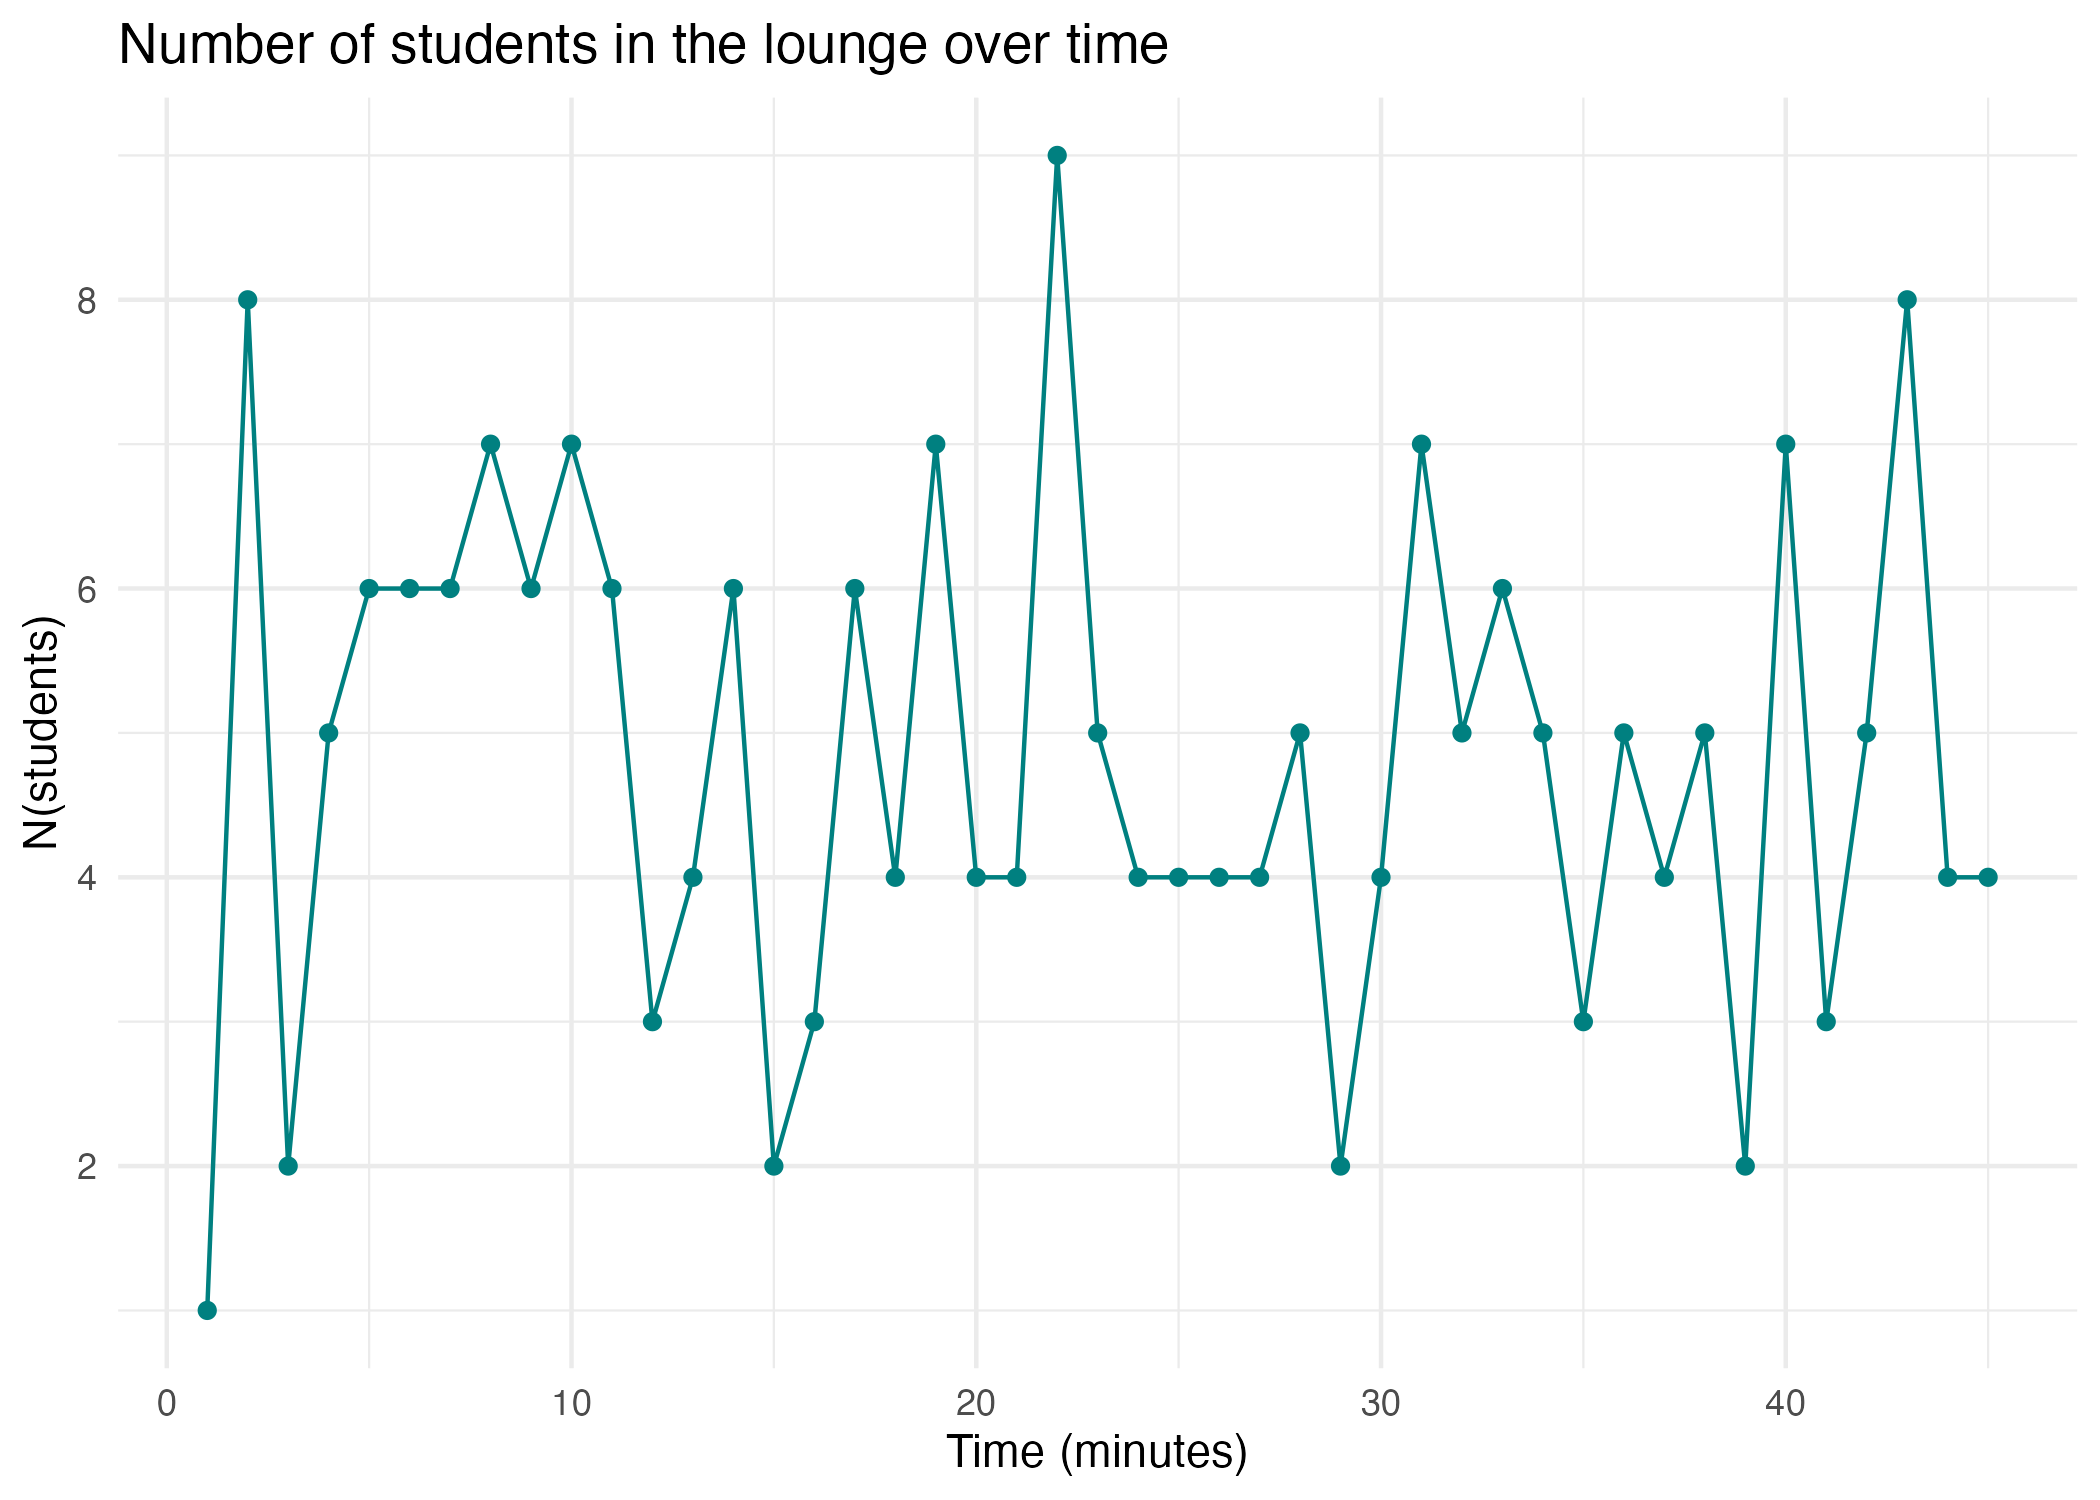
\includegraphics[width = 5in]{images/Fig1.png}
    \caption{Number of students in the lounge over time}
    \label{fig:nofood}
    \end{center}
\end{figure}


\subsection{Finding 2}

\begin{figure}[!htbp]
    \begin{center}
    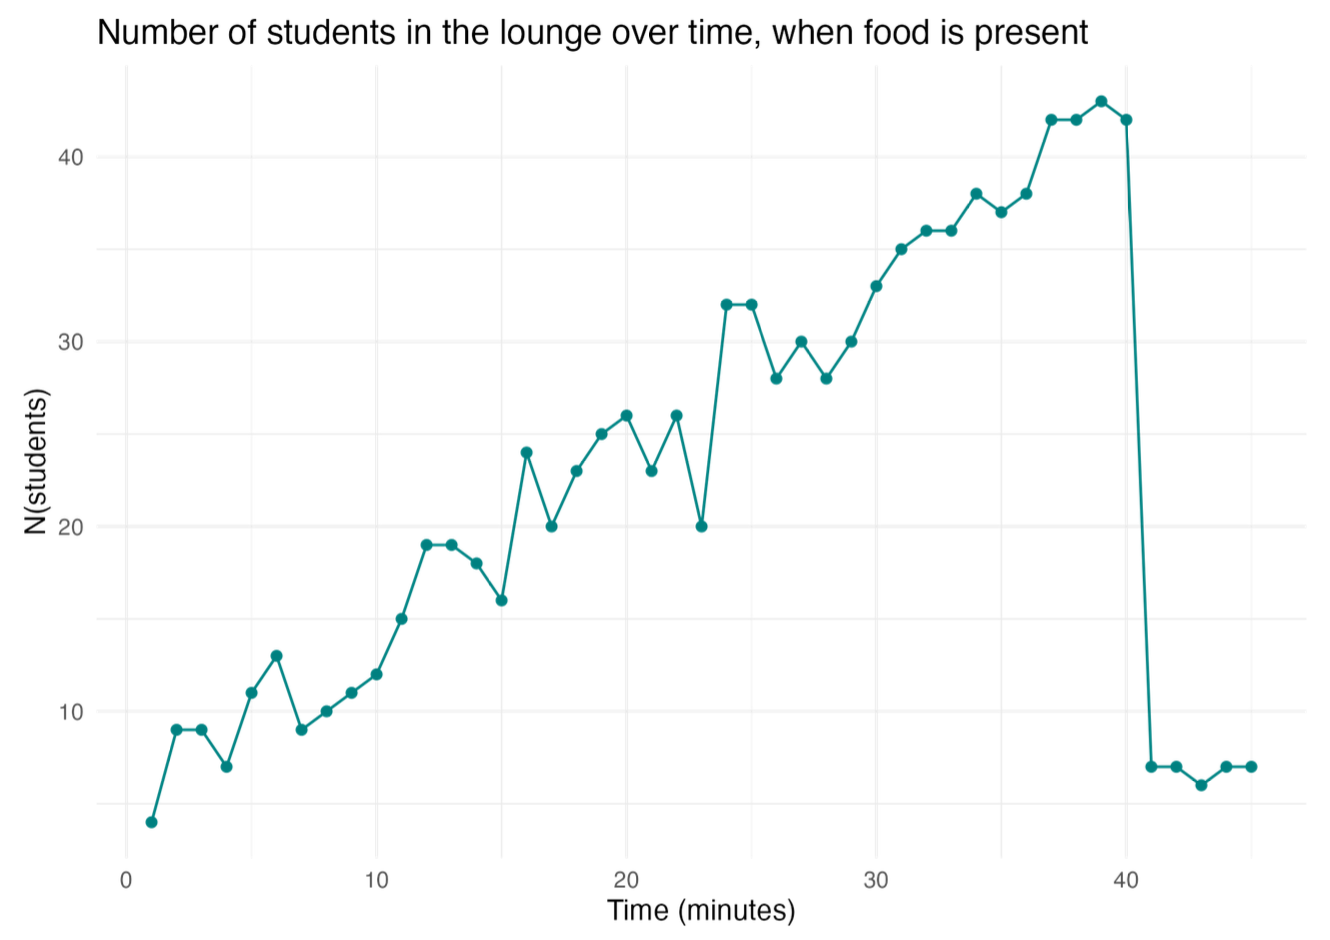
\includegraphics[width = 5in]{images/Fig2.png}
    \caption{Number of students in the lounge over time}
    \label{fig:yesfood}
    \end{center}
\end{figure}



\section{Discussion}
\label{discussion}

Take some time to write your discussion section, it should not be something you scramble to write right before you submit your draft. Instead, the Discussion is  where you connect your findings to previous literature and answer your research question.

You will also want to evaluate the strengths and weaknesses of your research in this section here

\section{Conclusion}
\label{conclusion}

In the conclusion, you shouldsummarize the main finding, and  1) discuss possible future directions, and/or 2) write about some implications of your work. If you'd prefer, you can incorporate this final section into \autoref{discussion}.

\vfill
{\normalsize \section*{Data and Code Availability Statement}}

Include your Data/Code availability statement here, including a link to a repository/GitHub repo as appropriate.
\href{https://github.com/UC-MACSS/example/}{Here} is the example of a GitHub repo we used in our Perspectives class, and \href{https://social-science-data-editors.github.io/guidance/Requested_information_dcas.html}{here} is more information regarding data availability statements.

\newpage
\section*{References}
\label{references}
\printbibliography[heading=none]

\newpage
\section*{Appendix}
\label{app}

You shouldn't need an appendix, but if you do you can add it to the end of the document.
You can link to it throughout the document like this: \nameref{app}


\end{document}








